\documentclass[12pt,a4paper]{article}
\usepackage[left=2cm,right=2cm,top=2cm,bottom=2cm]{geometry}


%idioma
\usepackage[utf8]{inputenc}
\usepackage[spanish]{babel}

%hipervinculos
\usepackage{hyperref}

%gráficos
\usepackage{graphicx}
% % % % % % % % % % % % % % % % % % % % % % Fuentes piola


\usepackage{cmbright}


%Bibtex
\usepackage[numbers]{natbib}



            
%%%%%%%%%%%%%%%%%%%%%%%%%%%%%%%%%%%%%%%%%%%%%%%%  
%Microtype = estilo más refinado (?)
\usepackage[protrusion=true,expansion=true]{microtype}
%\usepackage{microtype}%Estandar

%%%%%%%%%%%%%%%%%%%%%%%%%%%%%%%%%%%%%%%%%%%%%%%%  
%Gráficos
\usepackage{graphicx}

%%%%%%%%%%%%%%%%%%%%%%%%%%%%%%%%%%%%%%%%%%%%%%%%  
%Tablas
\usepackage{multirow}
\usepackage{tabularx} %tablas con mucho texto
\usepackage{booktabs}


%%%%%%%%%%%%%%%%%%%%%%%%%%%%%%%%%%%%%%%%%%%%%%%%  
% Cabecera y pie de página
\usepackage{fancyhdr}

\pagestyle{fancy}
\fancyhf{} %Limpia las cabeceras
\renewcommand{\headrulewidth}{0pt}
\fancyhead[L]{\footnotesize\bfseries  [75.06] Organización de Datos}
%\fancyhead[C]{}
\fancyhead[R]{\footnotesize\bfseries  Diseño TP - Grupo 20}

\fancyfoot[L]{}
\fancyfoot[C]{\thepage}
\fancyfoot[R]{}
\renewcommand{\headrulewidth}{0.4pt}
\renewcommand{\footrulewidth}{0.6pt}

%%%%%%%%%%%%%%%%%%%%%%%%%%%%%%%%%%%%%%%%%%%%%%%%  
%Contador de secciones empieza en 0
%\setcounter{section}{-1}

%%%%%%%%%%%%%%%%%%%%%%%%%%%%%%%%%%%%%%%%%%%%%%%%  
%Fin declaraciones

\begin{document}
\bibliographystyle{plainnat}

\section{Introducción}

El objetivo de este Trabajo Práctico es realizar un programa que permita buscar frases en un conjunto de documentos (la colección).

Para ello, luego de investigar sobre el tema, concluimos que la estructura más popular para este tipo de aplicación es el índice invertido, que consiste de dos grandes componentes: el vocabulario de términos (por ejemplo, de palabras) de la colección, y una lista invertida, la cual es una estructura que contiene información sobre la ocurrencia (o posición) del término.

Para la búsqueda de frases en índices invertidos se han propuesto diferentes enfoques. La primera estrategia, propuesta en \citet{Williams99what'snext?} (\citeyear{Williams99what'snext?}) sería guardar palabras contiguas, en lo que se llama un índice de próxima palabra (nextword index). En la frase <<hoy hace calor>> se guardarían <<hoy hace>> y <<hace calor>> acompañado del documento en donde aparecen. Este enfoque podría utilizar hasta aproximadamente el doble de espacio en disco que la colección, porque se guardan todas las palabras de los documentos en dúos que pueden tener muy poca repetición. Se crean índices, aunque de tamaño considerable, de rápido accionar para encontrar frases.

Otra estrategia, la que utilizaremos, es almacenar la posición de cada término en cada documento de forma ordenada, así pueden utilizarse distintos algoritmos de compresión. Para buscar una frase, primero se buscan todas las palabras que contiene y se obtienen las listas invertidas para cada una, extrayendo las posiciones y documentos en donde aparecen las mismas. Luego, aplicando un algoritmo de intersección, se filtran los documentos en donde las palabras efectivamente existen en el orden deseado.

Una última estrategia, bastante más sofisticada, sería la presentada por \citet{Williams:2004:FPQ:1028099.1028102} (\citeyear{Williams:2004:FPQ:1028099.1028102}) en donde se hace una combinación de las anteriores (un índice invertido con las palabras menos comunes y un indice de próxima palabra con los dúos más comunes) pero agregando un índice con las frases más comunes. Esta aproximación acelera un 400 \% el tiempo de búsqueda sobre nuestra propuesta, pero ocupa el doble de espacio en disco, según el mismo artículo. Como priorizamos espacio antes que tiempo, la idea es descartada.




\section{Definiciones básicas}

Para diagramar el trabajo primero estableceremos las siguientes definiciones básicas:
\begin{itemize}

%\item Consulta (q): es una ni idea que poner

\item Documento: conjunto de datos en formato estándar de texto (Unicode).

\item Carpeta a indexar: es la que se le pasa al programa creado para que procese todos sus documentos, y permita hacer consultas sobre su contenido

\item Colección: conjunto de todos los documentos que aparecen en la carpeta a indexar.

\item Diccionario: conjunto de todos los términos.

\end{itemize}


%\subsection{Término (\textit{\textnormal{T}})}
\subsection{Término (\textnormal{\itshape T})}

 
Se considera término \textit{T} a todo conjunto de caracteres alfanumérico sumados al apóstrofo (o comilla simple: ' ). Cada término es, o bien, una cantidad numérica desde 1 (una) hasta una cantidad no definida de cifras, o bien palabras tanto simples como compuestas. Se desarrolla sobre este tema en la Sección \ref{sec:parser}.


\subsection{docID (\textnormal{\itshape D})}
\noindent (\textit{document identification} = identificador de documento)

Este es un número asignado unívocamente a cada documento de la carpeta a indexar. Para hacer este proceso, se listan recursivamente todos los documentos (que se suponen \textit{indexables}, es decir, de texto plano) y se los ordena (el criterio será develado más adelante). Este orden otorga el docID de cada documento, que comienzan desde el 1 (uno).


\subsection{d-gap}
\noindent(\textit{document-gap} = distancia entre documentos)

Considerando una lista de docIDs en orden ascendente, se puede almacenar la misma con el primer elemento seguido de las diferencias entre los elementos siguientes, los \textit{d-gaps}. Se utiliza la definición dada en \citet[p.~115]{WittenMoffatBell99}.

Por ejemplo $\langle 1, 2, 4 , 5 , 8 \rangle$ se puede transformar en $\langle 1, 1, 2 , 1 , 3 \rangle$.



%\citeauthor[p.~115]{WittenMoffatBell99}.

%\subsection{Frecuencia absoluta (\textnormal{\itshape F \texorpdfstring{\textsubscript{F}})}}
\subsection{Frecuencia absoluta (\texorpdfstring{$F_{T}$}{FF})}

Cantidad de veces que aparece un término \textit{T} en toda la colección.


%\subsection{Frecuencia relativa (\textnormal{\itshape f \texorpdfstring\textsubscript{D,T}})}
\subsection{Frecuencia relativa (\texorpdfstring{$F_{D,T}$}{FFD})}

Cantidad de veces que aparece un término \textit{T} en un documento \textit{D}.

\subsection{Lista de posiciones}

También llamada lista de ocurrencias. Es aquella que almacena las posiciones $p_i$ en un documento \textit{D} en donde aparece el término \textit{T}. Una posición en un documento corresponde a la cantidad de términos hasta el término en consideración, empezando por el 1.
%\begin{center}
%    \includegraphics[scale=0.8]{./images/graf9}
%    
\includegraphics[width=0.4\textwidth]{./images/logoFiubaCompleto}
%\end{center}

\section{Generación de términos}\label{sec:parser}
 
Todos los términos estarán compuestos de una única palabra y se guardarán en el Diccionario con letras minúsculas. Se tomaron decisiones basándonos en las siguientes directivas.


\subsection{No se guardarán términos de más de una palabra}

Aunque los indices tipo Nextword (próxima palabra) son capaces de otorgar velocidades de acceso superiores a los índices invertidos tradicionales, ocupan en promedio un 60 \% del espacio de la colección, según mencionan \citet{Williams99what'snext?} (\citeyear{Williams99what'snext?}). 

Para este Trabajo Práctico, se construirá un índice preparado para buscar frases, pero a través de sus posiciones. Esto quiere decir que se tendrán en cuenta la separación entre palabras dentro de un documento. Por ejemplo un sustantivo propio de más de una palabra como <<San Francisco>> se separará en dos términos <<San>> y <<Francisco>>. Al hacer la consulta el programa calculará la distancia entre las dos palabras: (<<San>>, posición $i$) y (<<Francisco>>, posición $i+1$), con las cuales se podrá intersecar con las listas invertidas de cada una y filtrar los documentos en donde en aparecen juntas en las posición requerida.


\subsection{Se guardarán todos los términos en letra minúscula}
En un texto, puede haber palabras que contengan mayúsculas en los siguientes casos:

%comiencen con una letra mayúscula solo en 2 casos:

\begin{itemize}
\item Mayúscula al comenzar la palabra: porque es un sustantivo propio
\item Mayúscula al comenzar la palabra: porque está precedida por un punto <<.>>
\item Mayúscula en medio de la palabra: porque es un código o abreviatura (<<IQJ653>>, <<PhD>>)
\end{itemize}

Esto sería un problema si quisiéramos guardar términos de más de una palabra como en el ejemplo anterior ya que se complicaría enormemente para identificar <<San Francisco>> en el siguiente escenario: <<… buenos momentos. San Francisco es …>>. No hay forma de saber si <<San>> empieza con mayúscula porque es un sustantivo propio o porque está al lado de un punto. Por suerte, esto no será un problema, ya que se guardará todo en minúsculas.

Que todo se guarde en minúsculas, también ayuda en la búsqueda, ya que el usuario del programa podría escribir de forma incorrecta sin poner las mayúsculas e igualmente encontrar lo que busca.

 
 
\subsection{Casos particulares de signos de puntuación}
 
\begin{itemize}

\item Guiones: si se encuentra un guion (medio o bajo) se toma como si fuese un espacio. Si el guion está dividiendo 2 palabras, se guarda cada palabra por separado como un término. También se reemplazan por espacios las ‘@’ y los ‘/’.

\item Apóstrofo (o comilla simple): por estar los textos de la colección en idioma inglés, conviene contemplar algunos casos del uso del apóstrofo y como se los tratará, a través de los siguientes ejemplos:
\begin{itemize}

\item  <<Grey’s Anatomy>>: en este caso, se guardarán los términos <<grey's>> y <<anatomy>> por separado.
\item  <<Isn’t it?>>: se guardará <<isn't>> y <<it>>.
\item  <<Baba O’Riley>>:  se guardará <<baba>> y <<o'riley>>.
\item  Caracteres que se ignoran: todos los caracteres que no son alfanuméricos y <<encierran>> conjuntos de palabras como son \texttt{¿?¡!()[]{}}, comillas dobles, acentos graves y agudos.
% ’’. 
También se ignoran \texttt{.:,;~ * \^{} +- \$ \#} .

\end{itemize}

\end{itemize}

\subsection{Números}

Los números se guardarán como términos comunes y silvestres. Por ejemplo:

\begin{itemize}
\item <<1000>> $\Longrightarrow$ <<1000>>
%\item <<1.000>> $\Longrightarrow$ <<1.000>>
\item <<03/04/2004>> $\Longrightarrow$ <<03>>, <<04>> y <<2004>>
\end{itemize}

%etc
%\section{Construcción del índice: primera parte}

Se mostrará la creación del índice a través de un ejemplo: se quiere indexar la carpeta <<vainilla/>> la cual contiene 3 documentos.

\begin{figure}[!h]
\centering
    
\includegraphics[scale=0.9]{./Images/vainillaDir.png}
\caption{Ejemplo de directorio de trabajo}
\label{fig:directorioTrabajo}
\end{figure}


\subsection{Lectura del directorio y asignaciones de docIDs}

Luego de verificar que el directorio a indexar existe, se leen los nombres de \textbf{todos} los documentos del mismo (consideramos que el directorio es de \textit{buena fe}), incluyendo los contenidos en carpetas interiores. Se ordenan los nombres alfabéticamente y se les asigna un docID correlativamente con el orden, es decir, el archivo que queda con el nombre en primera posición tiene el docID más bajo, el cual en el esquema propuesto por nosotros, es 1 (uno). Así se sigue hasta el último documento.

\subsection{Extracción de términos y creación del índice en memoria}

\begin{figure}[!h]
\centering
    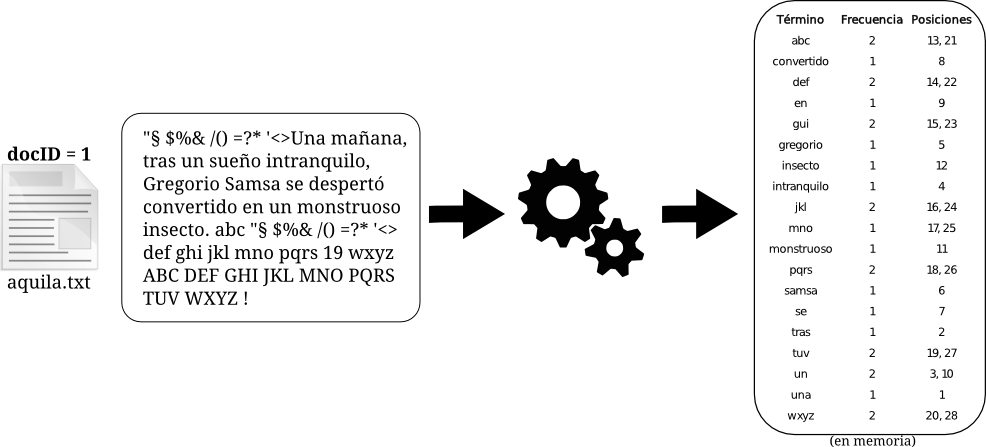
\includegraphics[scale=0.9]{./Images/parseoYMem.png}
\caption{Un archivo procesado y cargados sus términos en memoria}
\label{fig:parseoymem}
\end{figure}

Como mencionamos en la Sección \ref{sec:parser} cada término es una palabra o cifra numérica. El programa crea listados en memoria principal con la siguiente información: para un término $T_i$ se almacena que aparece en el documento con docID $D_1$ en las posiciones $p_1, p_2, p_3 \ldots p_m$, y listados equivalentes para los demás documentos. La estructura de estos listados es:

\[
\left\lbrace T_i ;
    \left( D_1 , 
        \left\langle
            p_1, p_2, p_3 \ldots p_m 
        \right\rangle  
    \right)
    ;
    \left( D_2 , 
        \left\langle
            p_1, \ldots p_f
        \right\rangle  
    \right) 
    ;
    \ldots
    ;
    \left( D_j , 
        \left\langle
            \dots
        \right\rangle  
    \right) 
\right\rbrace 
\]

Este procedimiento (generar términos y llevarlos a memorias principal) se hace constantemente hasta que ocurra uno de los siguientes hechos:

\begin{enumerate}
\item Se terminen de procesar todos los documentos
\item Se ocupe toda la memoria dedicada para el programa (se requerirán 512 MB de RAM dedicados, es decir, una PC con al menos 1 GB en total). En tal caso se crearán archivos temporales, se vaciará la memoria y se vuelve al paso 1.
\end{enumerate}


\subsection{Creación de archivos temporales}

La primera vez que ocurra uno de estos dos momentos se creará un directorio temporal <<vainillatemp/>> que irá guardando archivos temporales con la información tal cual aparece en memoria. Sucesivas bajadas de memoria a disco, generarán archivos temporales de nombre incremental.

\begin{figure}[!h]
\centering
    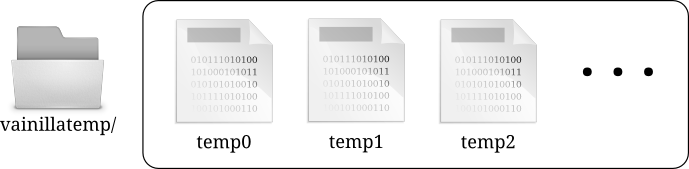
\includegraphics[scale=0.9]{./Images/tempDirEstr.png}
\caption{Un directorio temporal con archivos temporales}
\label{fig:tempdir}
\end{figure}


Cada archivo temporal contiene información suficiente para armar un índice por si mismo, ya que almacena para los documentos procesados, los términos, docIDs, frecuencias relativas y lista de posiciones como se muestra en la Figura \ref{fig:tempfile}.


\begin{figure}[!h]
\centering
    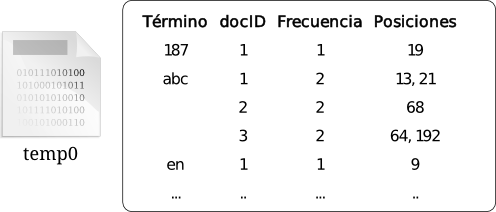
\includegraphics[scale=0.9]{./Images/tempFileEstr.png}
\caption{Datos almacenados en un archivo temporal}
\label{fig:tempfile}
\end{figure}


%\begin{figure}[here]
%\includegraphics[width=0.9\textwidth]{images/JobInformationDialog.jpg}
%\caption{A prototype of the Job Information dialog}
%\label{fig:jobInformationDialog}
%\end{figure}
%\include{Referencias}




\bibliography{Referencias}

\end{document}
